\documentclass[12pt]{article}
\usepackage{dsfont}
\usepackage{amsmath}
\usepackage[margin=2.5cm]{geometry}
\usepackage{amssymb}
\usepackage{mathtools}

\DeclarePairedDelimiter\ceil{\lceil}{\rceil}
\DeclarePairedDelimiter\floor{\lfloor}{\rfloor}

\usepackage{algorithm}
\usepackage[noend]{algpseudocode}
\usepackage{pgf}
\usepackage{tikz}
\usepackage{tikz-qtree}
\usepackage{graphicx}

\title{\textbf{CSC373 - Problem Set 4}}
\author{Authors: Luke Bacchus, Naslin Rahman, Zhuoqian Li}
\date{\today}

\begin{document}
\maketitle
\section*{Question 1}
Given $F = (V, E)$, we define $F'$ with exactly the same edges and vertices $(V, E)$, and for every edge $e \in E$ where the capacity of $e \in F$ is $cap(e)$ we let $e$'s capacity in $F' = cap(e) * (|E| + 1) + 1$.  We observe that $(S, T)$ is an $s$-$t$ cut of $F$ if and only if it is also a $s$-$t$ cut of $F'$, because $F$ and $F'$ have exactly the same edges and vertices. 
\newline \,
\newline Claim: If $(S, T)$ is a non minimal cut of $F$, then $(S, T)$ is a non minimal cut of $F'$. \newline \,
\newline Let $(S', T')$ be a minimal cut of $F$ with $cap(S', T') = K$ in $F$. For any non minimal cut $(S, T)$, we must have that $cap(S, T) \geq K + 1$ (since all the weights are integral). $cap(S', T') = K * (|E| + 1) + k'$ in $F'$, where $k'$ is the number of crossings between $S'$ and $T'$. On the other hand, we must have that $cap(S, T) \geq (K + 1) * (|E| + 1) + k$, where k is the number of crossings between $S$ and $T$ . We know that both $k$ and $k'$ are in the range $1$ to $|E|$. We can see that $cap(S', T') < cap(S, T)$ in $F'$. Therefore $(S, T)$ is not a minimal cut of $F'$.
\newline \, 
\newline
Now we can observe that any minimal cut of $F'$ must be a minimal cut of $F$ by contraposition. Consider two minimal cuts of $F$, $(S_1, T_1)$ and $(S_2, T_2)$. The capacity of these cuts is equal to $K * (|E| + 1) + k_1$ and $K * (|E| + 1) + k_2$ in $F'$ where $k_1$ and $k_2$ are the number of crossings between each cut. Therefore, the minimum cut of $F'$ must be a minimum cut of $F$ that has a minimal number of crossings.
\newline \, \newline
So, to compute a minimum cut of $F$ that has a minimum number of crossings, one constructs $F'$ and finds a minimum cut in $F'$ in polynomial time. This cut is the required answer.
\newline This question was written and read by  Luke, Naslin, and Zhuoqian.

\newpage

\section*{Question 2}
\begin{enumerate}
    \item[a.] Graph for max flow and min cut:\\
        
        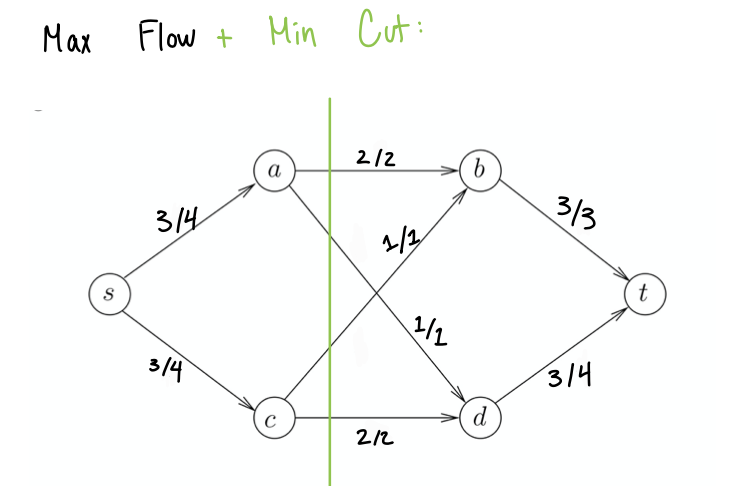
\includegraphics[width=8cm]{Graphs/2A.png}

        This is correct due to the Ford Fulkerson Algorithm, which outputs a maximum flow and (A,B) is a min cut.

    \item[b.]  Residual Graph of Flow Network:

        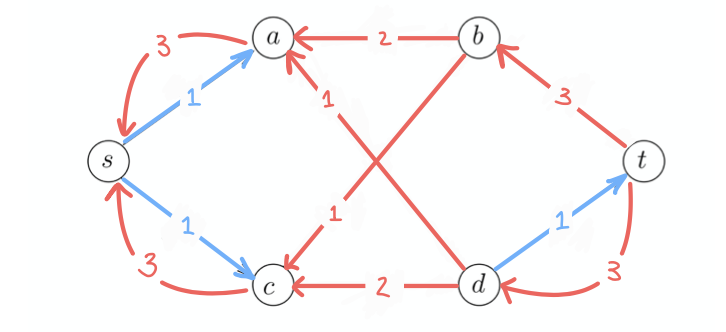
\includegraphics[width=8cm]{Graphs/2B.png}

    \item[c. ]Set of bottleneck edges: {(c,d),(a,d)}
    \item[d. ] Simple flow network with no bottleneck edges
    
        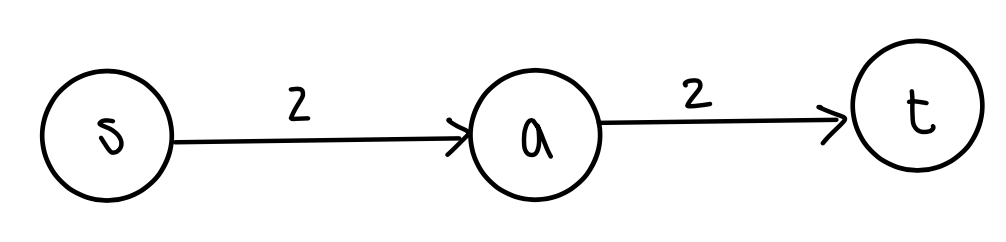
\includegraphics[width=6cm]{Graphs/2C.png}

    \item[e. ] Find the maximum flow f of (G, s, t, c), and its corresponding residial
               graph $G_{f}$.
               
               To find a bottleneck edge, we want to find a path from s to t where all edges still
               have space left except for on edge. 
               

               Algorithm: Starting from edge s, explore other nodes connected to this node with
               an edge from the node. (Ex: Explore node u if there is an edge (s,u)).

               Choose one node to further explore at a time, and keep track of unexplored nodes
               in an array so you can return at a later time. Along with these 
               unexplored nodes, keep track the number of edges along the path to that node
               who do not have an edge value in Gf, meaning that f(e) = c(e)
               in the max flow graph. These edges can be visualized by the blue arrows as seen in 2b.

               If this number exceeds 2, then this is an invalid path and return 
               to the most previous unexplored node. If the node t is reached, and the number
               of these kind of edges is exactly one, then that edge is a bottleneck edge.

               If we are on a path with a previously found bottleneck edge, we do not need to 
               continue exploring. Continue until all possible paths are explored to get all possible bottleneck edges.

               $\\$
               $\\$
               Correctness:

               Let BE represent the be the set of bottleneck edges by the algorithm for (G,s,t,c).

               Let BE* be the actual set of bottle neck edges for (G,s,t,c).

               Assume $BE != BE*$.

               Case 1: $\exists (u,v) \in E s.t.  (u,v)\in BE$ and $(u,v) \notin BE*$
               This would mean that the algorithm found an edge (u,v) that is not actually a 
               bottleneck edge. 
               
               If the algorithmn found (u,v) it would mean that there exists a path from s to t where for 
               every e in the path except for (u,v), f(e) $<$ c(e). And f((u,v)) = c((u,v)) on the 
               max flow graph. Thus, increasing its capcity where c'((u,v)) $>$ c((u,v)) would increase 
               the value of a maximum flow of (G,s,t,c').

               Thus, meaning that (u,v) is a bottleneck edge, which results in a contradiction.

               Case 2: $\exists (u,v) \in E s.t.  (u,v)\notin BE$ and $(u,v) \in BE*$
               This would mean that there is a bottleneck edge that was not found by the algorithmn.
               
               For this to be possible, it would mean that for all the paths from s to t that contain (u,v), a) (u,v) 
               had an edge in $G_f$ or b) another edge on that path did not have an edge in $G_f$.

               In case a), this would mean that on those paths, f((u,v)) $<$ c((u,v)) in the max flow graph. 
               It would mean that raising the capacity of (u,v) would not increase the value of a maximum 
               flow of (G,s,t,c') since there is a restriction elsewhere. 

               In case b), this would mean that for those paths, even if you raised c((u,v)),
               there is another edge limiting the flow of that path to t. 

               Both cases would contradict the definition of a bottleneck edge. Meaning that the algorithmn
               must've found (u,v)


               Both cases result in a contradiction so our assumtion that $BE != BE*$ is false.

               $\\$
               $\\$
               Runtime: O((m+n)C) to run the Ford-Fulkerson Algorithmn, and O((m+n)C) for the worst case of
               the runtime of any possible path from s to t with max C iterations. Checking $G_{f}$ is constant.

               Thus, O((m+n)C).

               This question was written and read by  Luke, Naslin, and Zhuoqian.
\end{enumerate}
\newpage
\section*{Question 3}
    We will reduce the regular edge-disjoint problem done in lecture. First create a new graph called $G'$ that is created as follows: For each node u of G (excluding s and t), we will create 2 new nodes (u1) and (u2) in $G'$. Then in $G'$ put a directed edge from (u1) to (u2) with weight 1. Then for each each (u,v) in G, we put an edge from (u2) to (v1) with weight of 1. All edges that start with s becomes (s, v1) and ones that end with t become (v2, t).
    \\\\
    Example: \\
    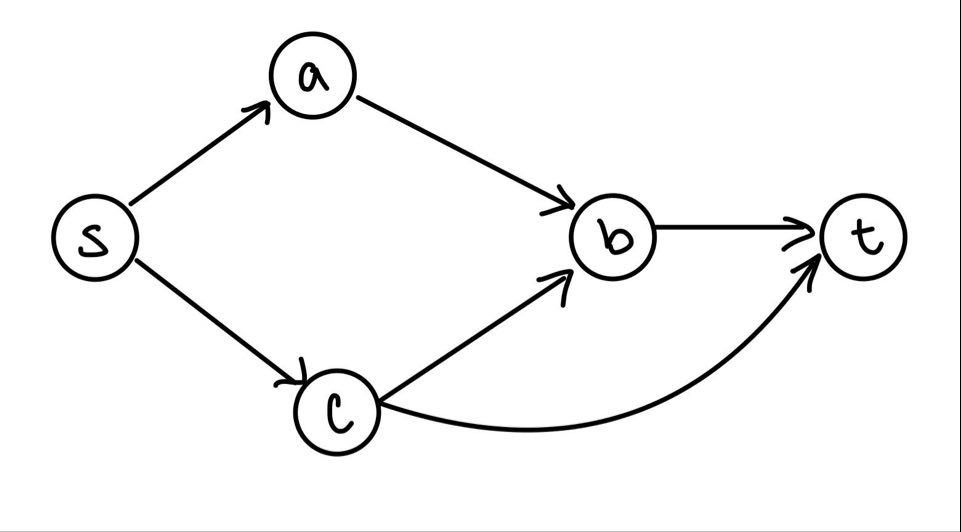
\includegraphics[width=8cm]{Graphs/3A.jpg}
            
    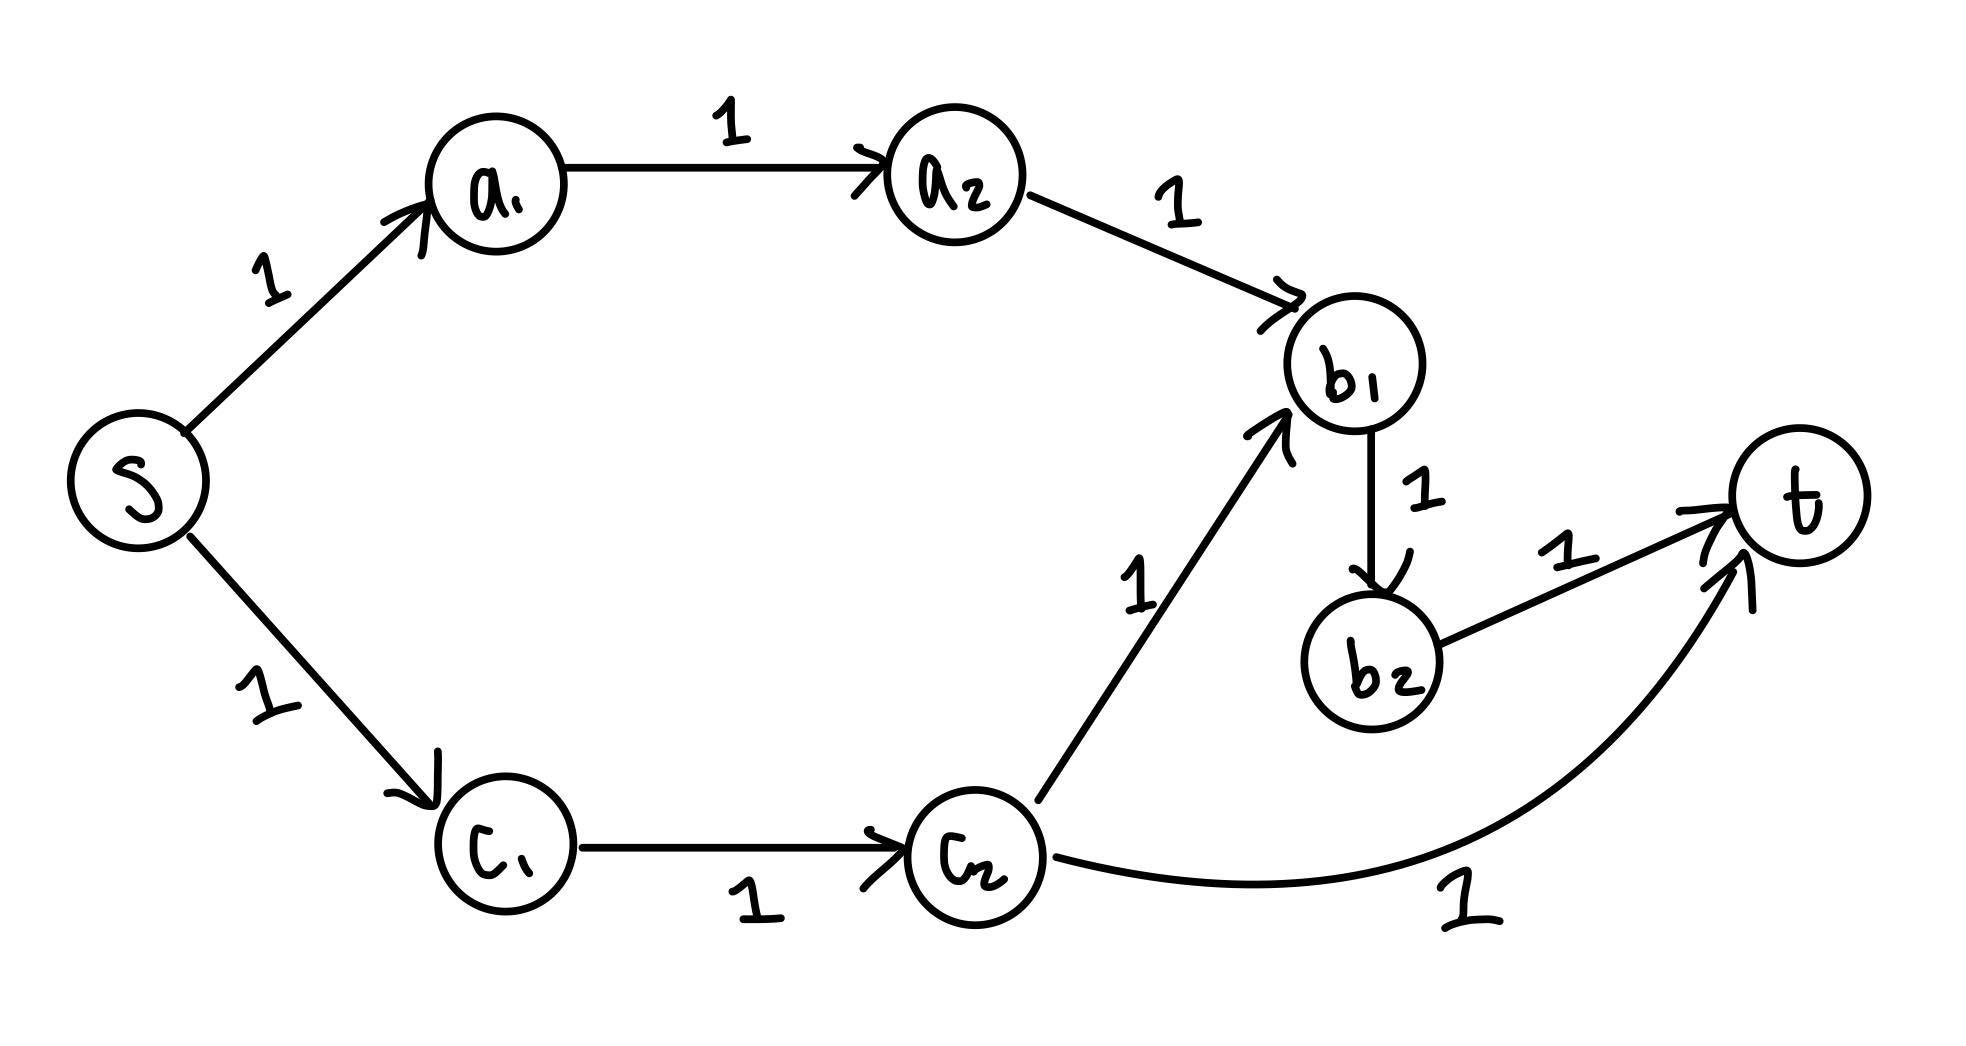
\includegraphics[width=8cm]{Graphs/3B.jpg}
    \\\\
    Now if we find a max flow of $G'$ using Ford Fulkerson we get the max size set of node-disjoint $s->t$ paths. 
    This algorithm works because each vertex in the original graph becomes an edge in the new graph so running the algorithm to find the max number of edge-disjoint paths will give us the our answer. No two $s->t$ paths cans share a vertex because then more than 1 $s->t$ path can have an edge from u1 to u2. From lecture we know if there are k edge-disjoint $s->t$ paths in G then there is an integral flow of value k so we need to find the the max value of k using Ford Fulkerson's algorithm.
    \\
    Time Complexity: Our new graph $G'$ with $n'$ nodes and $m'$ edges will have 2*(n-2) vertices and m+(n-2) edges. \\ Step 1: Creating this graph will be $O(2*(n-2) + m+(n-2)$ which is $O(n + m)$ \\
    Step 2: Constructing the flow network (with all weights = 1) which is $O(n + m)$\\
    Step 3: Finding the max flow of $G'$ using FF which is O(m'* n') = $2(n-2) * m+(n-2)$ which is $O(n^2 + nm)$\\
    Step 4: Path decomposition which is $O(n + m)$\\
    \newline Total Runtime $O(n^2 + mn)$
    \newline This question was written and read by  Luke, Naslin, and Zhuoqian.



\end{document}